\documentclass[11pt]{article}

\usepackage{amsmath}
\usepackage{amssymb}
\usepackage[margin=0.68in]{geometry}
\usepackage{booktabs}
\usepackage{enumitem}
\usepackage{fancyhdr}
\usepackage{graphicx}
\usepackage[table]{xcolor}
\usepackage[hidelinks]{hyperref}
\usepackage{listings}
\usepackage{microtype}
\usepackage{tabularx}
\usepackage{tikz}
\usepackage{titlesec}
\usetikzlibrary{arrows.meta,positioning}
\graphicspath{{docs/lessons/assets/}{../assets/}}

\definecolor{AdkBlue}{HTML}{24577A}
\definecolor{AdkRed}{HTML}{A23B32}
\definecolor{AdkGreen}{HTML}{39734C}
\definecolor{CodeGray}{HTML}{F7F7F7}
\hypersetup
{
    pdftitle={ADK Lesson 012: Tabletop Traffic Junction},
    pdfauthor={Kevin Shanahan},
    pdfsubject={Deterministic traffic state machines, safe actuation, shift-register display, and circuit-native evidence},
    pdflang={en-US}
}
\pagestyle{fancy}
\fancyhf{}
\lhead{\textsc{ADK Lesson 012}}
\rhead{Tabletop Traffic Junction}
\cfoot{\thepage}
\setlength{\headheight}{14pt}
\setlength{\parindent}{0pt}
\setlength{\parskip}{5pt}
\setlist{nosep,leftmargin=1.45em}
\titleformat{\section}{\Large\bfseries\color{AdkBlue}}{\thesection}{0.5em}{}
\titleformat{\subsection}{\large\bfseries\color{AdkBlue}}{\thesubsection}{0.5em}{}
\lstdefinestyle{adkcpp}
{
    language=C++,
    backgroundcolor=\color{CodeGray},
    basicstyle=\ttfamily\footnotesize,
    keywordstyle=\color{AdkBlue}\bfseries,
    commentstyle=\color{AdkGreen},
    columns=fullflexible,
    keepspaces=true,
    showstringspaces=false,
    frame=single,
    rulecolor=\color{black!20},
    breaklines=true,
    tabsize=4
}
\newcommand{\checkbox}{\(\square\)}
\newcommand{\blank}[1]{\rule{#1}{0.4pt}}
\newcommand{\warningbox}[1]{%
  \begin{center}
  \fcolorbox{AdkRed}{AdkRed!6}{\parbox{0.91\linewidth}{\textbf{\color{AdkRed}Safety checkpoint.} #1}}
  \end{center}}
\newcommand{\evidencebox}[1]{%
  \begin{center}
  \fcolorbox{AdkBlue}{AdkBlue!5}{\parbox{0.91\linewidth}{#1}}
  \end{center}}

\begin{document}

\begin{center}
  {\Huge\bfseries Tabletop Traffic Junction}\\[4pt]
  {\Large Observe, decide, actuate---without conflicting greens}\\[8pt]
  \textit{The signal heads reveal the state machine; the display reveals its time.}
\end{center}

\begin{tabularx}{\linewidth}{@{}>{\bfseries}l X >{\bfseries}l X@{}}
Lesson & 012 --- integration project & Time & 180--240 minutes\\
Prerequisites & Lessons 001--011 & Board & Arduino Mega 2560\\
Evidence & two signal heads, pedestrian pair, countdown, test points &
Status & host verified; physical acceptance open\\
Safety & E1 tabletop model; USB-powered current-limited LEDs only\\
\end{tabularx}

\warningbox{This model is not a road controller and must never direct real
traffic. Disconnect USB before wiring. Every LED and display segment needs its
own resistor. Use only the Mega's 5\,V rail. Stop for heat, odor, resets,
unexpected simultaneous greens, or disagreement between the schematic and
breadboard. Remove USB power to stop the experiment.}

\section{Mission and evidence chain}

Build two vehicle signal heads, a pedestrian request and signal pair, and a
one-digit countdown. The project composes:

\[
\text{button}\rightarrow\texttt{TrafficInput}\rightarrow
\texttt{TrafficJunction}\rightarrow\texttt{TrafficSignals}\rightarrow
\text{current-limited LEDs}
\]
\[
\texttt{nextDeadline}\rightarrow\texttt{SevenSegmentDisplay}\rightarrow
\texttt{ShiftRegisterOutput}\rightarrow\text{visible digit}.
\]

The D13 board LED turns on only after every first-class object initializes, so
it is the acquisition indicator. The heads are the primary diagnostic channel.
All-red plus pedestrian stop is the visible safe state. The countdown is
independent supporting evidence: it shows the remaining whole seconds until
the next transition. Serial is not required. Named electrical test points are
D30 (main red), D32 (main green), D33 (side red), and D35 (side green), each
measured relative to GND.

By the end, you can:

\begin{itemize}
  \item explain why a hardware-neutral state engine receives explicit time;
  \item trace a latched pedestrian request until it is served;
  \item prove from observations that both greens are never active together;
  \item explain why actuation turns permissive signals off before changing red;
  \item relate a semantic glyph to an atomic 74HC595 latch update;
  \item distinguish successful acquisition, a commanded all-red state, and a
        measured electrical all-red state.
\end{itemize}

\section{System composition}

\begin{center}
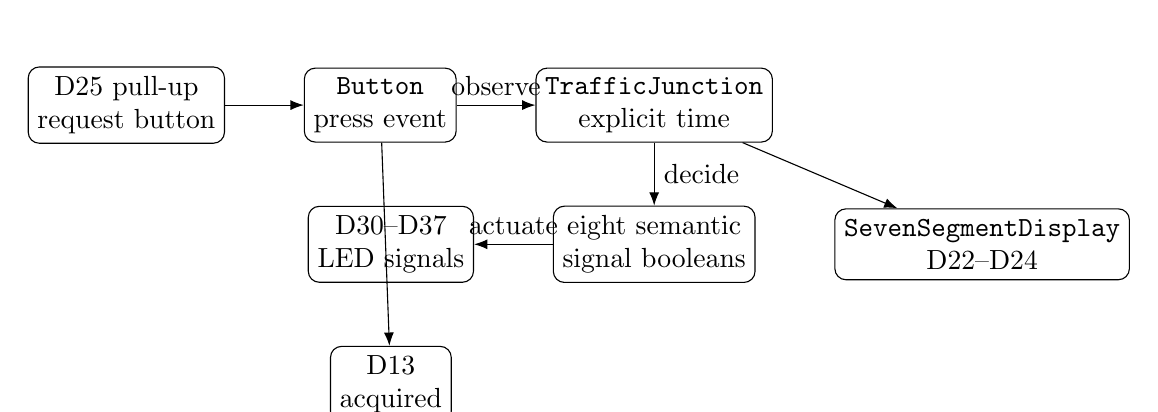
\begin{tikzpicture}[
    node distance=8mm and 10mm,
    box/.style={draw,rounded corners,minimum height=9mm,align=center},
    >=Latex]
  \node[box] (button) {D25 pull-up\\request button};
  \node[box,right=of button] (observe) {\texttt{Button}\\press event};
  \node[box,right=of observe] (engine) {\texttt{TrafficJunction}\\explicit time};
  \node[box,below=of engine] (signals) {eight semantic\\signal booleans};
  \node[box,left=of signals] (heads) {D30--D37\\LED signals};
  \node[box,right=of signals] (display) {\texttt{SevenSegmentDisplay}\\D22--D24};
  \node[box,below=of heads] (acquire) {D13\\acquired};
  \draw[->] (button) -- (observe);
  \draw[->] (observe) -- node[above]{observe} (engine);
  \draw[->] (engine) -- node[right]{decide} (signals);
  \draw[->] (signals) -- node[above]{actuate} (heads);
  \draw[->] (engine) -- (display);
  \draw[->] (observe) -- (acquire);
\end{tikzpicture}
\end{center}

The canonical sketch follows the same narrative. \texttt{loop()} observes one
button event, asks the engine to decide, then actuates the returned snapshot.
It never invents signal combinations in Arduino-facing code.

\subsection{The state promise}

\begin{tabularx}{\linewidth}{@{}l X X@{}}
\toprule
Phase & Vehicle indication & Pedestrian indication\\
\midrule
\texttt{AllRed} & both red & stop\\
\texttt{MainGreen}/\texttt{MainYellow} & named main aspect; side red & stop\\
\texttt{SideGreen}/\texttt{SideYellow} & named side aspect; main red & stop\\
\texttt{PedestrianWalk} & both red & walk\\
\texttt{PedestrianClearance} & both red & stop\\
\texttt{Fault} & both red & stop\\
\bottomrule
\end{tabularx}

A request is an event, not a held electrical level. The engine latches an
accepted request and serves it after the side phase. A circuit-health failure
latches \texttt{Fault}; only a new, explicit \texttt{initialize()} starts a new
run. No call blocks while a phase elapses.

\section{Orientation drawing}

\begin{figure}[ht]
  \centering
  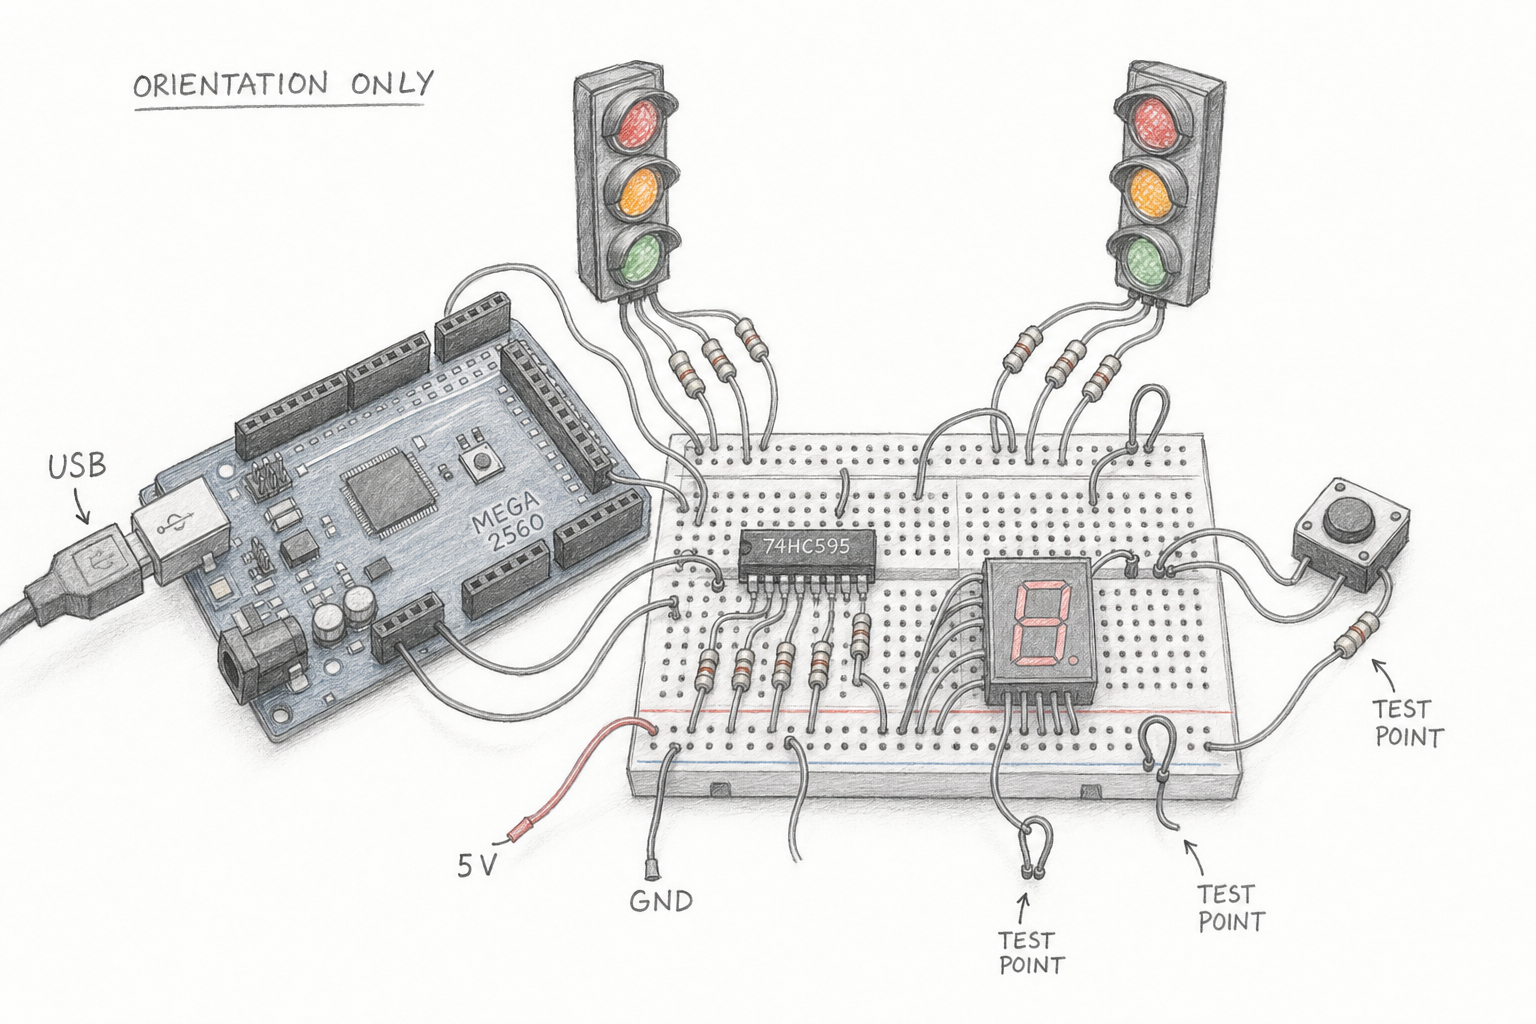
\includegraphics[width=0.94\linewidth]{012-traffic-junction-pencil.png}
  \caption{Pencil orientation of the Mega, two model heads, request button,
  shift register, display, and test points. It is not an authoritative wiring
  diagram. Breadboard connectivity and package pin order are simplified; use
  the literal connection table and each part's identified datasheet.}
\end{figure}

\section{Parts, limits, and literal wiring}

\begin{tabularx}{\linewidth}{@{}l l X@{}}
\toprule
Quantity & Part & Requirement\\
\midrule
1 & Mega 2560 & USB powered\\
1 & 74HC595 & identified pinout; 0.1\,\(\mu\)F local decoupling\\
1 & one-digit display & common cathode, identified segment pinout\\
8 & signal LEDs & two red/yellow/green heads plus red/green pedestrian pair\\
15 & resistors & 330\,\(\Omega\) per signal LED; 1\,k\(\Omega\) per display segment\\
1 & momentary button & normally open\\
1 & multimeter & unpowered continuity and powered DC voltage\\
\bottomrule
\end{tabularx}

\textbf{Mega and signal connections.}

\begin{tabularx}{\linewidth}{@{}l l X@{}}
\toprule
Function & Mega pin & Literal path\\
\midrule
request & D25 & D25 to button to GND; internal pull-up\\
acquisition & D13 & built-in LED; on only after every object initializes\\
main head & D30/D31/D32 & pin to 330\,\(\Omega\) to red/yellow/green anode;
                              every cathode to GND\\
side head & D33/D34/D35 & same order and resistor rule\\
pedestrian & D36/D37 & walk green/stop red, each through 330\,\(\Omega\)\\
\bottomrule
\end{tabularx}

\textbf{74HC595 and display connections.}

\begin{tabularx}{\linewidth}{@{}l l X@{}}
\toprule
Function & Connection & Required interpretation\\
\midrule
serial data/clock/latch & D22 to DS, D23 to SHCP, D24 to STCP &
  \texttt{ShiftRegisterPins\{22,23,24\}}\\
control & MR to 5\,V; OE to GND & never leave either floating\\
power & VCC to 5\,V; GND to GND; 0.1\,\(\mu\)F across them &
  place capacitor at the IC\\
segments & Q0--Q6 to a--g, Q7 to decimal point &
  each path has its own 1\,k\(\Omega\) resistor\\
display return & both common cathodes to GND & verify the exact package pinout\\
\bottomrule
\end{tabularx}

Do not copy a display pin number from the pencil drawing. Identify the part and
check continuity unpowered. With a conservative 3\,mA per lit display segment
and 10\,mA per signal LED, the worst expected visible state is under 55\,mA;
record actual resistor values, forward voltages, and measured current before
claiming that budget.

\section{Build and run from the CLI}

\begin{lstlisting}[style=adkcpp]
make arduino-Lesson012TrafficJunction
make upload-Lesson012TrafficJunction PORT=/dev/ttyACM0
make monitor-describe PORT=/dev/ttyACM0
make serial-log PORT=/dev/ttyACM0 \
    SERIAL_LOG=build/evidence/lesson012-optional.log
\end{lstlisting}

Serial capture is optional context. The required proof is the visible and
electrical evidence below. Build and upload targets must remain the canonical
path; no IDE-specific step is part of the lesson.

\subsection{The narrative run loop}

\lstinputlisting[
  style=adkcpp,
  firstline=47,
  lastline=69,
  caption={Canonical observe--decide--actuate flow.}
]{examples/Lesson012TrafficJunction/Lesson012TrafficJunction.ino}

The engine's \texttt{TrafficSignals} is the sole actuator model. The
\texttt{showSignals()} adapter first removes green, walk, and yellow permission;
then it establishes all-red; only then does it present the requested state.
This sequencing prevents a valid semantic snapshot from becoming a transient
conflicting-green electrical command.

\section{Predict, observe, interpret}

\begin{tabularx}{\linewidth}{@{}p{0.21\linewidth} X X@{}}
\toprule
Predict & Observe & Interpret\\
\midrule
Acquisition completes & D13 turns on & every project object initialized; this
does not prove the signal pin levels\\
Startup is all-red & both red heads and pedestrian stop illuminate before any
green & the first semantic state was actuated; measure test points before
calling it electrical proof\\
Only one vehicle direction proceeds & watch an entire main/side cycle; compare
D32 and D35 & any simultaneous high reading is a stop condition and a failed
acceptance test\\
One request is remembered & press and release D25 once during main green; wait
without holding it & a later pedestrian walk proves event capture and latching\\
The display changes atomically & watch the countdown at a phase boundary &
mixed or torn segments indicate wiring, resistor, or latch trouble\\
Failure is all-red & use the host fault fixture; do not create shorts on the
powered circuit & fault snapshots command two reds and pedestrian stop\\
Shutdown is electrically inactive & upload a dedicated acceptance sketch that
calls endpoint shutdown; measure each named pin & high impedance is distinct
from the running model's commanded all-red state\\
\bottomrule
\end{tabularx}

\evidencebox{\textbf{Do not merge three claims.} D13 proves completed
acquisition. D30/D32/D33/D35 measurements establish the commanded electrical
levels. A separate shutdown measurement establishes endpoint high impedance.
Record all three independently.}

\section{Deterministic desk experiment}

Before wiring, replay this trace on paper. Use the configured phase durations
from the canonical source.

\begin{enumerate}
  \item At \(t=0\), initialize. Record phase, all eight signals, and deadline.
  \item Update immediately before and exactly at the startup deadline.
  \item During main green, supply one \texttt{pedestrianRequestEvent=true}.
        Return it to false on the next update.
  \item Advance exactly to each deadline through main yellow, clearance,
        side green, side yellow, clearance, walk, and pedestrian clearance.
  \item At every row, evaluate
        \(\neg(\texttt{mainGreen}\land\texttt{sideGreen})\).
  \item Repeat the identical trace. Snapshots must match byte for byte.
\end{enumerate}

\begin{tabularx}{\linewidth}{@{}l l l l l X@{}}
\toprule
Time & Input event & Expected phase & Main & Side & Pedestrian/pending\\
\midrule
\blank{0.7in} & \blank{0.55in} & \blank{0.9in} &
\blank{0.55in} & \blank{0.55in} & \blank{1.1in}\\
\blank{0.7in} & \blank{0.55in} & \blank{0.9in} &
\blank{0.55in} & \blank{0.55in} & \blank{1.1in}\\
\blank{0.7in} & \blank{0.55in} & \blank{0.9in} &
\blank{0.55in} & \blank{0.55in} & \blank{1.1in}\\
\blank{0.7in} & \blank{0.55in} & \blank{0.9in} &
\blank{0.55in} & \blank{0.55in} & \blank{1.1in}\\
\bottomrule
\end{tabularx}

\section{Diagnosis}

\begin{tabularx}{\linewidth}{@{}l X X@{}}
\toprule
Observation & Likely layer & Next bounded check\\
\midrule
No LEDs and blank display & power or acquisition & remove USB; inspect rails,
polarity, pin map, and resource conflicts\\
Heads correct, digit wrong & display encoding/wiring & run lesson 010; compare
Q0--Q7 with a--g/decimal point\\
Digit tears during change & latch wiring & inspect STCP D24 and shared ground;
do not add delays to hide it\\
Request never served & button/event path & observe raw D25 and repeat lesson
003 debounce evidence\\
Both greens visible & actuator wiring or severe defect & remove USB
immediately; unpowered continuity from D32/D35 to the intended LEDs\\
All-red forever & startup/fault/configuration & reproduce the same timestamps
in host tests and inspect \texttt{status}\\
Unexpected resets & current or wiring & remove USB; measure resistors and
inspect for rail shorts before reapplying power\\
\bottomrule
\end{tabularx}

\section{Exercises}

\begin{enumerate}
  \item Add a host trace with a request one millisecond before a deadline.
        State exactly which snapshot accepts it and why.
  \item Prove that every path from one green direction to the other contains
        \texttt{AllRed} for at least \texttt{vehicleAllRed}.
  \item Replace the numeric countdown with \texttt{Dash} during fault. Keep the
        heads as the authoritative safe-state evidence.
  \item Design a maintenance self-test that illuminates one aspect at a time.
        It may run only from all-red and must return to all-red on every error.
  \item Calculate measured LED current from resistor voltage, then compare the
        sum with your predicted current budget.
\end{enumerate}

\section{Bench acceptance record}

\textbf{This source has host and compile evidence only. Physical acceptance is
deferred until a completed, reviewed record is committed.}

\begin{tabularx}{\linewidth}{@{}l X l X@{}}
Date & \blank{1.2in} & Reviewer & \blank{1.3in}\\
Board/revision & \blank{1.2in} & Supply/USB source & \blank{1.3in}\\
Meter & \blank{1.2in} & Firmware commit & \blank{1.3in}\\
74HC595 marking & \blank{1.2in} & Display marking & \blank{1.3in}\\
\end{tabularx}

\begin{itemize}
  \item[\checkbox] Unpowered continuity matches every literal connection.
  \item[\checkbox] Every signal resistor measures \blank{0.7in};
        every segment resistor measures \blank{0.7in}.
  \item[\checkbox] Startup visibly reaches all-red before a green.
  \item[\checkbox] D13 turns on only after full acquisition.
  \item[\checkbox] D32 and D35 are never simultaneously high over three cycles.
  \item[\checkbox] One short D25 press is eventually served exactly once.
  \item[\checkbox] The digit changes without a visible intermediate pattern.
  \item[\checkbox] Maximum measured signal current is \blank{0.6in} mA;
        display current is \blank{0.6in} mA; total is \blank{0.6in} mA.
  \item[\checkbox] Running fault indication is all-red plus pedestrian stop.
  \item[\checkbox] Separate shutdown firmware leaves output pins measured
        high impedance.\par Method/result: \blank{2.2in}.
  \item[\checkbox] Reset and USB removal produce no observed conflicting green.
\end{itemize}

Deviations and observations:

\vspace{0.55in}
\hrule
\vspace{0.55in}
\hrule

\section{What to carry forward}

The reusable idea is not ``a traffic light.'' It is the boundary between a
deterministic decision and a transactional physical presentation. The engine
speaks in domain signals; endpoint-owning adapters perform safe ordering; the
circuit supplies evidence alongside its useful behavior. The same separation
supports later environmental, access, rover, greenhouse, telemetry, and inert
cue projects.

\textbf{Primary source paths:}
\href{https://github.com/spincyc/adk/blob/main/src/traffic_junction.h}
{Traffic junction API},
\href{https://github.com/spincyc/adk/blob/main/src/seven_segment_display.h}
{seven-segment API},
\href{https://github.com/spincyc/adk/blob/main/src/shift_register.h}
{shift-register API}, and
\href{https://github.com/spincyc/adk/tree/main/examples/Lesson012TrafficJunction}
{canonical example}.

\end{document}
